\documentclass[conference]{IEEEtran}
\IEEEoverridecommandlockouts

\usepackage{amsmath}
\usepackage{newtxtext,newtxmath}
\usepackage{graphicx}
\usepackage{booktabs}
\usepackage{siunitx}
\usepackage[hidelinks]{hyperref}
\usepackage{cite}

\graphicspath{{figures/}}

\begin{document}

\title{A Small Biped Picks Up an Unknown Payload\\[4pt] {\Large Randomize, Adapt, or Monitor?}}

\author{\IEEEauthorblockN{Shengwei Li}
\IEEEauthorblockA{The University of Sydney, NSW, Australia\\
Project technical report, November 2026}}

\maketitle

\begin{abstract}
A \SI{0.74}{kg} biped walks with a policy trained by reinforcement learning and picks up an object of unknown mass with its beak.
This report studies three questions in simulation.
First, when does a policy that never saw a payload fail? Its velocity drifts from \SI{20}{g} and it starts to fall at \SI{80}{g}, 11\% of the robot's mass.
Second, which training method handles the payload: randomizing it, giving the policy the true mass, or letting the policy adapt from a history of observations?
Randomization alone removes the falls inside the training range, at no cost without payload.
The other two do not track the commanded velocity better, but they keep the velocity constant as the payload changes; outside the training range, the history policy falls more often than the others.
Third, can a runtime monitor see that a payload is too heavy in time to prevent the fall?
The error of a learned one-step model raises an alarm 0.7--\SI{0.9}{s} before every fall at \SI{200}{g}, at a 5\% false-alarm rate; a threshold on the neck joint is \SI{0.3}{s} later and misses a quarter of the falls.
Standing still after the alarm does not help, but dropping the payload does, and only if the alarm is early.
All 17 expected outcomes were written down before their tests: 14 held, 2 failed, and 1 could not be tested as written.
\end{abstract}

\section{Introduction}

A locomotion policy trained by reinforcement learning (RL) is tuned to the robot it was trained on.
When the robot picks something up, its mass distribution changes and the policy acts on a body it does not know.
Three responses are common.
\emph{Randomize}: vary the payload during training, so that one policy works for all of them \cite{tobin2017domain,peng2018sim}.
\emph{Adapt}: let the policy infer the payload from its recent observations \cite{lee2020learning,kumar2021rma}.
\emph{Monitor}: accept that the policy has a limit, detect at runtime that the limit is exceeded, and do something safe \cite{sha2001simplex}.

This report compares the three on one small robot and one fault.
It is the second report in a line of work.
The first \cite{li2026arm} asked how a model predictive controller and an imitation policy on a robot arm fail under an unknown payload, and how a monitor can detect it.
Here the same question is put to a legged robot and an RL policy, and the monitoring tools are carried over.
The report has three parts:
\begin{itemize}
\item \textbf{Part I, the failure.} At what payload does a standard walking policy fail, and what degrades first?
\item \textbf{Part II, the methods.} Payload randomization (P1), a policy that is told the true mass (P2), and a policy with an observation history and an asymmetric critic (P3), each with three training seeds.
\item \textbf{Part III, the monitors.} Four signals, each with a threshold calibrated for a 5\% false-alarm rate, and two fallbacks: stand still, or drop the payload.
\end{itemize}

The main observations are:
\begin{enumerate}
\item Tracking fails before balance. The baseline policy loses most of its backward speed by \SI{60}{g} while it still almost never falls.
\item Randomization is enough inside its range and costs nothing without payload. Knowing the mass does not reduce the tracking error; it removes the dependence of the velocity on the payload.
\item The payload mass can be read linearly from the hidden layer of the history policy, but also from the policy without history. The information is in the current observation; what differs between the policies is whether training made them use it.
\item A learned one-step model is a better monitor than the obvious physical signal, because it is faster. The \SI{0.3}{s} it gains decide whether a fallback works.
\item The monitor detects ``outside the training range'', not ``about to fall'', so it stops many robots that would not have fallen.
\end{enumerate}
No new method is proposed. The contribution is a controlled comparison of known ingredients on a carefully modelled small robot, with the expected results fixed before the tests.

\section{Related Work}

\textbf{RL for legged locomotion.} Policies trained in massively parallel simulation \cite{rudin2022learning} with proximal policy optimization (PPO) \cite{schulman2017ppo} now transfer to real robots when the actuators are modelled well \cite{hwangbo2019learning} and the dynamics are randomized \cite{tobin2017domain,peng2018sim}.
We use mjlab \cite{zakka2026mjlab}, which runs MuJoCo \cite{todorov2012mujoco} on the GPU, with the PPO implementation of RSL-RL \cite{schwarke2025rslrl}.

\textbf{Adaptation.} A teacher policy with privileged information can be distilled into a student that sees only a history of observations \cite{lee2020learning}; RMA \cite{kumar2021rma} trains an adaptation module to estimate a latent encoding of the environment from that history.
An asymmetric actor-critic \cite{pinto2018asymmetric} gives the privileged information to the critic only and needs a single training run. We use this simpler variant for P3.
Linear probes \cite{alain2016understanding} test whether a quantity can be read from a network's internal activations.

\textbf{Runtime monitoring.} Recent monitors for learned manipulation policies use the consistency of the policy's own outputs \cite{agia2024sentinel} or uncertainty scores with conformal calibration \cite{angelopoulos2021gentle} on successful runs \cite{romer2025fiper,xu2025faildetect}.
The Simplex architecture \cite{sha2001simplex} switches from a high-performance controller to a trusted one when a monitor raises an alarm.
In \cite{li2026arm}, model residuals detected a payload on an arm and a model predictive controller took over.
A small biped has no such trusted controller, so the fallback here must be a simple action.

\section{Setup}
\label{sec:setup}

\subsection{Robot, task and baseline}

The robot is Microduck from Pollen Robotics \cite{pollen2026microduck}: about \SI{0.25}{m} tall, \SI{0.737}{kg} in the simulation model, with 14 position-controlled servos (five per leg, four in the neck and head).
We use the upstream velocity-tracking task on flat ground at a fixed commit and do not change it.
The upstream model includes a fitted servo model, observation noise and delays, and domain randomization of mass, joint friction and sensor errors.
The actor is a multilayer perceptron (512, 256 and 128 units) that maps 61 values (angular velocity, gravity direction, joint positions and velocities, the last action, and the commands) to 14 joint position targets at \SI{50}{Hz}. The critic also sees simulator state such as the base velocity and the foot contacts.

The baseline P0 is the upstream training run: 4096 parallel robots, 3000 iterations, \SI{2.4}{h} on one laptop GPU (RTX~5060, \SI{8}{GB}).
Without payload, P0 does not fall in 896 evaluation episodes, but it walks at only 50--60\% of the commanded forward speed and does not walk sideways. We checked this against the distance the robots covered; it is the behaviour of the policy.
Every comparison below is therefore made against a policy's own result without payload, and sideways commands are not used.

\subsection{Payload}

The robot holds a thin rod in its beak with a ball at the end, \SI{78}{mm} in front of the tip of the beak (Fig.~\ref{fig:setup}). The rod has no mass and nothing collides with the ball; only its mass and inertia act on the robot.
The payload appears \SI{5}{s} after the start of an episode, as if the robot picked it up.
Masses are 0 to \SI{200}{g} in nine steps. Because the beak is far in front of the feet, \SI{100}{g} moves the centre of mass of the whole robot \SI{19}{mm} forward.
The neck servos are soft, so the payload also pushes the head down, which moves the payload further forward.

\begin{figure}[t]
\centering
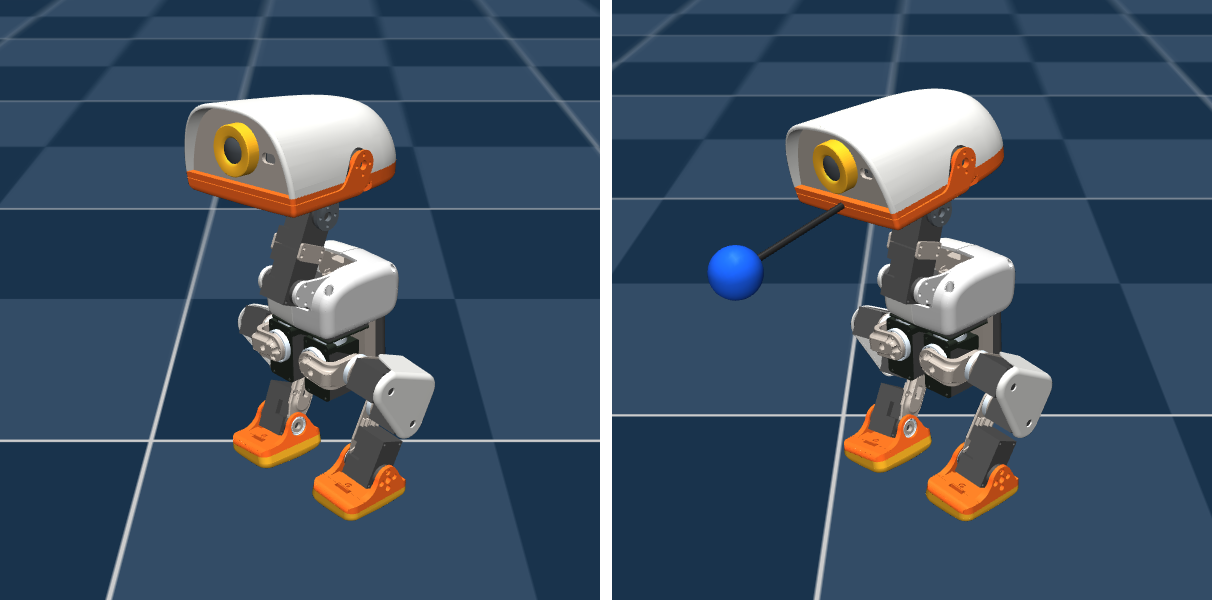
\includegraphics[width=\columnwidth]{setup}
\caption{The same robot (policy P1, command: stand) before the payload appears (left) and with \SI{100}{g} (right). The payload is the ball at the end of a massless rod. It pushes the head down, because the neck servos are soft.}
\label{fig:setup}
\end{figure}

\subsection{Evaluation}

The evaluation removes the training curriculum and the random pushes, so that a fall is caused by the payload. The other domain randomization stays on.
Each robot gets one of six fixed commands for a \SI{20}{s} episode: stand, forward slow (\SI{0.2}{m/s}), forward fast (\SI{0.4}{m/s}), backward (\SI{-0.3}{m/s}), turn (\SI{0.8}{rad/s}), and forward with a turn.
Tracking is measured from \SI{2}{s} after the payload appears.
A test uses seeds 2000 and 2001 with 64 robots per command and mass each: 768 episodes per mass and policy.
Repeating an evaluation with the same seed changes a fall rate by up to about 0.03 (the GPU simulation is not bit-reproducible), so smaller differences are not interpreted.

\begin{figure*}[t]
\centering
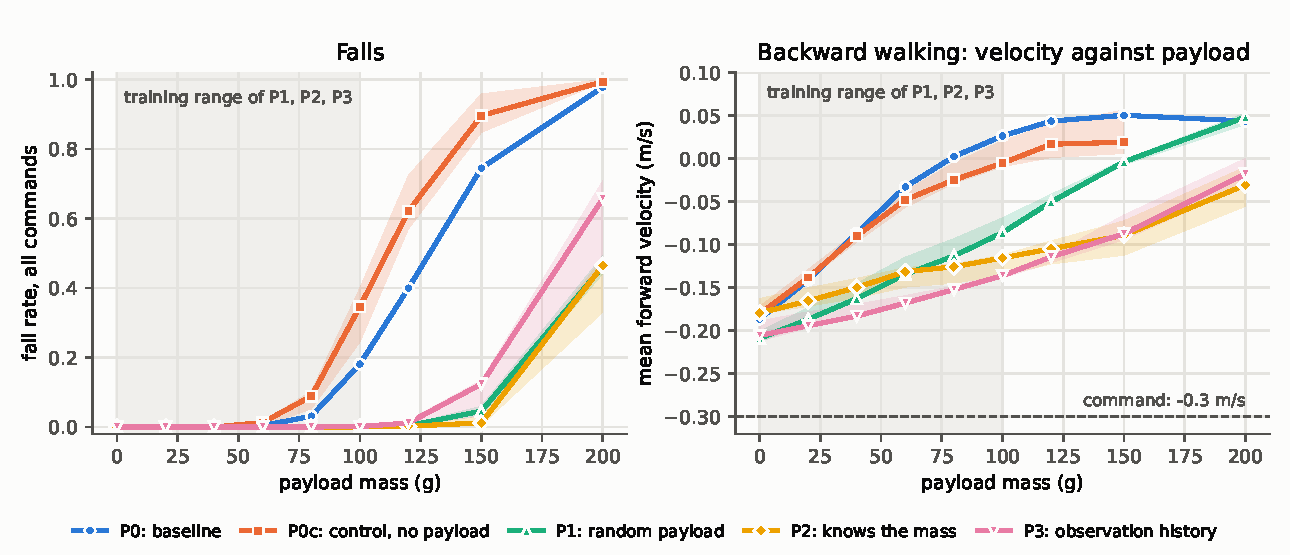
\includegraphics[width=\textwidth]{methods_test}
\caption{Parts I and II, test seeds 2000 and 2001, 768 episodes per mass and policy. Left: fall rate over all commands. Right: mean forward velocity with the backward command; a flat line means that the payload does not change how the robot walks. Lines are medians over three training seeds (P0: one), bands the range. At \SI{200}{g} all P0c robots fall before the measurement starts.}
\label{fig:methods}
\end{figure*}

\subsection{Methods}

All methods continue from the P0 checkpoint for 1000 more iterations (\SI{53}{min} each) with three training seeds (Table~\ref{tab:methods}).
During training the payload mass is drawn uniformly from the training range, and it appears at a random time.
P0c is a control that trains for the same additional time without payload; it separates the effect of the payload from the effect of more training.
P2 and P3 have a larger network input than P0. The new input weights start at zero, so both begin with exactly the behaviour of P0; we verified this in the simulator (largest action difference below \num{e-4}).
The first run of P3 collapsed within two iterations: the optimizer state for the 1464 new inputs had been set to zero, which made the first steps very large. Copying the state from the matching existing inputs fixed it.

\begin{table}[t]
\centering
\caption{Policies. All use the upstream network and reward.}
\label{tab:methods}
\footnotesize
\begin{tabular}{@{}lp{1.9cm}p{4.6cm}@{}}
\toprule
 & Training payload & Actor input\\
\midrule
P0 & none & 61 values (upstream)\\
P0c & none & as P0, trained longer (control)\\
P1 & 0--\SI{100}{g} & as P0\\
P2 & 0--\SI{100}{g} & as P0, plus the true payload mass\\
P3 & 0--\SI{100}{g} & the last 25 observations (\SI{0.5}{s}); only the critic sees the mass\\
\bottomrule
\end{tabular}
\end{table}

\subsection{Monitors and fallbacks}

For P1 and P3, an episode is \emph{normal} if the payload is inside the training range. A monitor should stay silent then and raise an alarm for a heavier payload.
Each monitor compares one signal per control step with a threshold:
\begin{itemize}
\item \emph{neck}: the position error of the neck joint, the obvious physical signal;
\item \emph{residual}: a small network (two hidden layers of 256 units) predicts the next measurement from the current observation and action; the signal is the size of its error. It is trained on about one million steps of normal episodes;
\item \emph{value}: the critic's estimate of future reward. The critic reads simulator state, and for P3 the true mass, so this signal is a reference, not something a real robot has;
\item \emph{probe}: the payload mass estimated by the linear probe of Section~\ref{sec:probe}.
\end{itemize}
Each signal is standardized on normal episodes of one development seed. The threshold is the split-conformal quantile \cite{angelopoulos2021gentle} of the largest value in each normal episode of a second development seed (2304 episodes), for a 5\% false-alarm rate per episode.
A third development seed was used to look at results and choose settings. The thresholds and models were committed before the tests.

At the first alarm the robot does one of two things. \emph{Stand}: the velocity command goes to zero. \emph{Drop}: the robot lets go of the payload, here without delay, which is the best case.

\subsection{Protocol}

Seeds are separated: 0--99 for training, 1000--1999 for development, 2000--2999 for tests.
Every setting was chosen on development seeds and then frozen.
Each expected outcome was written with a number and committed to the public repository before its test was run; Table~\ref{tab:hypotheses} lists all of them.
Results are the median over the three training seeds.

The code, the written expectations, the frozen monitor settings and every result file are public\footnote{\url{https://github.com/Shengwei-Li/microduck_control}}; the tables and figures of this report are generated from those files.
All training took about \SI{14}{h} on the laptop GPU (the baseline, and twelve runs of \SI{53}{min}); one evaluation of a policy over the nine masses takes about \SI{100}{s}.

\section{Part I: The Failure}
\label{sec:part1}

P0 never saw a payload. Fig.~\ref{fig:methods} (blue) shows its fall rate and Table~\ref{tab:hypotheses} the four expectations, all of which held.
The failure has two stages.
Up to \SI{60}{g} the robot almost never falls (4 of 768 episodes at \SI{60}{g}), but its velocity shifts forward: with the backward command it moves at \SI{-0.19}{m/s} without payload and \SI{-0.03}{m/s} with \SI{60}{g}, and with the fast forward command it speeds up from 0.21 to \SI{0.34}{m/s}.
From \SI{80}{g} it falls: 3\% at \SI{80}{g}, 18\% at \SI{100}{g}, 75\% at \SI{150}{g}.
The direction of motion matters. At \SI{120}{g}, 81\% of the robots walking fast forward fall, and 5\% of those walking backward.
A monitor that waits for a fall is therefore late in two ways: the policy has stopped doing what it was asked long before, and the fall itself comes quickly, a median of 1 to \SI{1.5}{s} after the payload appears (development seed).

\section{Part II: The Methods}
\label{sec:part2}

\subsection{Falls and tracking}

Table~\ref{tab:results} and Fig.~\ref{fig:methods} give the results.

\textbf{Randomization works, and more training does not.} P1 does not fall for any mass up to \SI{100}{g}. The control P0c is worse than P0 with a payload (35\% falls at \SI{100}{g} against 18\%); a possible reason is that longer training on the unloaded robot specialises the policy to it. The gain of P1 therefore comes from the payload in its training, not from the extra iterations.

\textbf{There is no cost without payload.} We expected P1 to track worse than P0c when unloaded, as the price of robustness. Its error is 0.5\% lower. Over this range of payloads, one policy can serve all of them.

\textbf{Knowing the mass does not improve tracking.} We expected P2, which is told the true mass, to track better than P1, and P3 to recover at least half of that gap. There is no gap: the errors of P1, P2 and P3 are within 4\% of each other, and P2 is not the lowest, so the expectation about P3 could not be tested as written.
The reason is in the baseline. All policies walk forward more slowly than commanded, and the payload pushes P1 forward, so for the forward commands the payload moves P1 \emph{towards} its command. The error measure rewards a drift that happens to have the right sign.

\textbf{What the mass does change.} The last two rows of Table~\ref{tab:results} measure how much the velocity changes between 0 and \SI{100}{g}. It changes least for P2, then P3, then P1, and every seed of P2 and P3 is below every seed of P1. A policy that knows or infers the payload walks the same way with and without it. This measure was not among the written expectations; it is an exploratory result that came from looking at why the expected gap was missing.

\textbf{Outside the range, adaptation is fragile.} We expected P3 to degrade more gracefully than P1 at \SI{150}{g}. It falls more often (12\% against 5\%), in two of its three seeds; the third is as good as P1. P1 and P2 do not differ outside the range.

\begin{table}[t]
\centering
\caption{Part II, test seeds, 768 episodes per mass and policy. Velocity change: mean forward velocity at \SI{100}{g} minus at \SI{0}{g}.}
\label{tab:results}
\footnotesize
\setlength{\tabcolsep}{4pt}
\begin{tabular}{@{}lcccc@{}}
\toprule
 & P0c & P1 & P2 & P3\\
\midrule
Fall rate at 100 g & 0.346 & 0.000 & 0.000 & 0.001\\
Fall rate at 150 g & 0.896 & 0.046 & 0.012 & 0.124\\
Fall rate at 200 g & 0.993 & 0.462 & 0.465 & 0.658\\
\midrule
RMSE at 0 g (m/s) & 0.180 & 0.180 & 0.181 & 0.180\\
RMSE, 20--100 g (m/s) & 0.193 & 0.161 & 0.163 & 0.158\\
\midrule
Velocity change, backward (m/s) & 0.175 & 0.127 & 0.051 & 0.067\\
Velocity change, forward fast (m/s) & 0.172 & 0.108 & 0.019 & 0.047\\
\bottomrule
\end{tabular}

\end{table}

\subsection{Is the payload mass in the network?}
\label{sec:probe}

If P3 adapts, the payload mass should be readable from its activations. We fit a linear model from the 128 outputs of the actor's last hidden layer to the mass in grams, on one development seed, and score it on the test seeds (payloads in the training range, from \SI{2}{s} after the payload appears).
For P3, $R^2$ is 0.86 in each of the three seeds, above the expected 0.7.

The comparison that was not an expectation is more informative. The same probe on P1, which has no history and no mass input, gives 0.83 (Fig.~\ref{fig:probe}).
The mass is therefore in a single observation: the payload bends the soft neck, and the joint positions show it.
P1 has this information and its velocity still drifts with the payload; P3 has it and does not drift.
The difference between them is not what the network can know but what training made it use, and the critic of P3 was given the mass.
A probe shows that information is present; it does not show that it is used.
Fig.~\ref{fig:probe} also shows that P3 is slower: one second after the payload appears, the probe on P1 has almost reached its final accuracy, while P3 still has old observations in its history.

\begin{figure}[t]
\centering
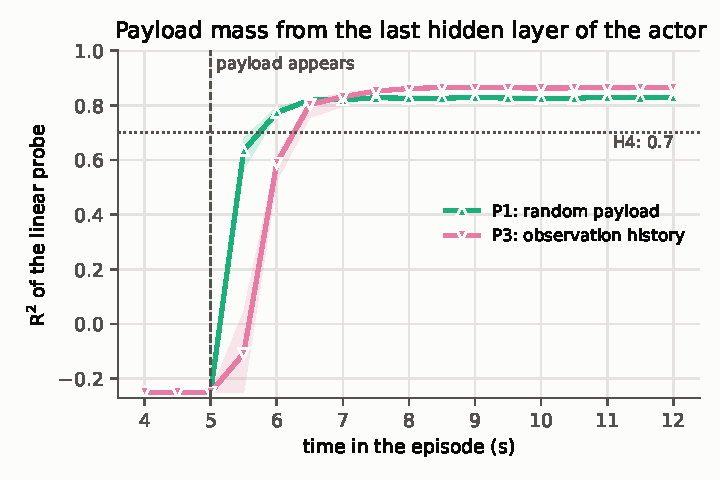
\includegraphics[width=\columnwidth]{probe_test}
\caption{Part II. $R^2$ of a linear probe for the payload mass on the last hidden layer of the actor, at each time in the episode, fitted on a development seed and scored on the test seeds. Before the payload appears the probe cannot know the mass and $R^2$ is negative (values below $-0.25$ are drawn at $-0.25$).}
\label{fig:probe}
\end{figure}

\begin{figure*}[t]
\centering
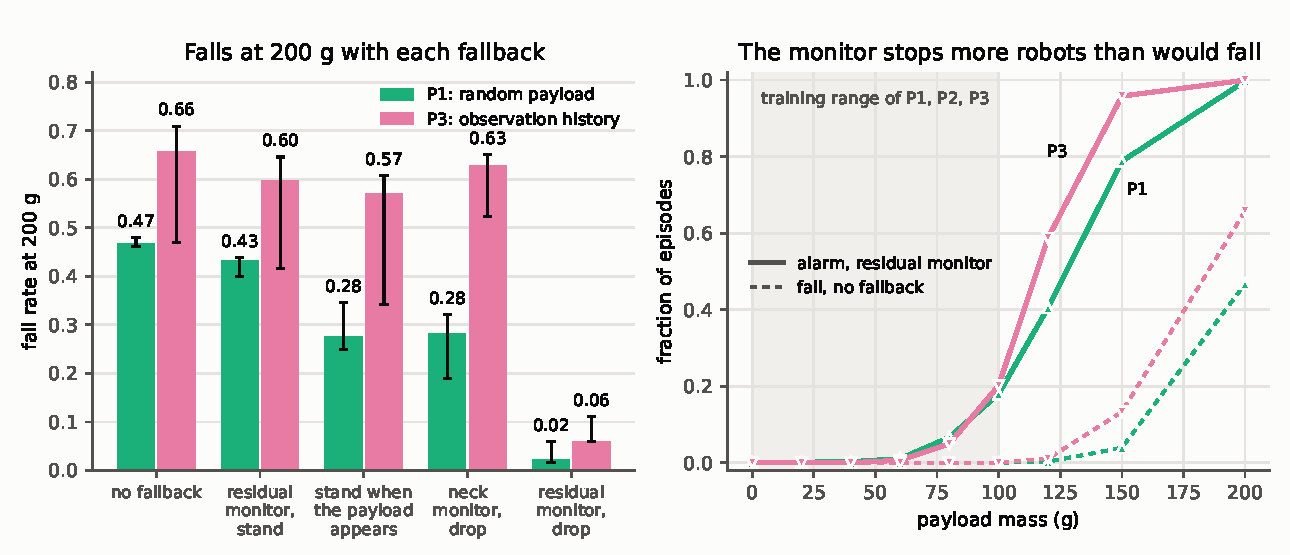
\includegraphics[width=\textwidth]{monitors_test}
\caption{Part III, test seeds 2000 and 2001. Left: fall rate at \SI{200}{g} with each monitor and fallback; bars are medians over three training seeds, error bars the range. Right: how often the residual monitor raises an alarm (target false-alarm rate 5\%), against how often the robot falls without a fallback.}
\label{fig:monitors}
\end{figure*}

\section{Part III: Monitors and Fallbacks}
\label{sec:part3}

\subsection{Detection}

Table~\ref{tab:monitors} gives the monitors at \SI{200}{g}, where P1 falls in 47\% and P3 in 66\% of the episodes.

\textbf{The calibration holds.} On the test seeds the false-alarm rates are 4.5--5.7\%, for a 5\% target.

\textbf{The learned residual catches every fall; the neck signal does not.} The residual monitor raises its alarm about \SI{0.3}{s} after the payload appears and before every fall in all six policies, a median of 0.74 (P1) and \SI{0.90}{s} (P3) ahead.
The neck monitor is \SI{0.3}{s} later and is ahead of only 74\% of the falls.
The neck is a soft joint; it takes time to bend, and some robots fall first.
After two seconds the neck error is a very clean measure of the mass, which is why the probe works, but a monitor is judged in the first second.

\textbf{The value signal is fastest, with privileged inputs.} For P1 the critic's value drops \SI{0.2}{s} after the payload appears, earlier than the residual. Its inputs include the base velocity and the foot contacts, which the robot does not measure. For P3 the critic sees the mass itself, and its alarm after \SI{0.02}{s} is not a detection.

\textbf{The probe is a weaker monitor on the policy it came from.} For P3 it catches 95\% of the falls. Far outside the training range the hidden layer no longer changes linearly with the mass: at \SI{200}{g} the estimate for one seed fell back to \SI{36}{g} on a development seed.

Accumulating the signals with CUSUM \cite{page1954cusum}, which was necessary on the arm \cite{li2026arm}, did not help: with a small allowance the alarm was seconds late, with a large one it equalled the plain threshold. The fault here is sudden and large.

\begin{table}[t]
\centering
\caption{Part III. Monitors on the test seeds. False-alarm rate on episodes with 0--\SI{100}{g}; the other rows at \SI{200}{g}. Caught: falls with an alarm before the fall. Lead time: alarm to fall. Delay: payload to alarm.}
\label{tab:monitors}
\footnotesize
\setlength{\tabcolsep}{4pt}
\begin{tabular}{@{}llcccc@{}}
\toprule
 & & neck & residual & value & probe\\
\midrule
P1 & False-alarm rate & 0.052 & 0.045 & 0.050 & 0.057\\
 & Falls caught & 0.74 & 1.00 & 1.00 & 1.00\\
 & Lead time (s) & 0.58 & 0.74 & 0.80 & 0.66\\
 & Delay (s) & 0.62 & 0.32 & 0.20 & 0.34\\
\midrule
P3 & False-alarm rate & 0.050 & 0.045 & 0.049 & 0.054\\
 & Falls caught & 0.74 & 1.00 & 1.00 & 0.95\\
 & Lead time (s) & 0.70 & 0.90 & 1.18 & 0.82\\
 & Delay (s) & 0.68 & 0.30 & 0.02 & 0.30\\
\bottomrule
\end{tabular}

\end{table}

\subsection{Fallback}

\textbf{Standing still does not help.} With the residual monitor and the stand fallback, the fall rate at \SI{200}{g} goes from 0.47 to 0.43 for P1 and from 0.66 to 0.60 for P3 (Table~\ref{tab:fallback}, Fig.~\ref{fig:monitors}).
This is not the monitor's fault. Even if every robot stands from the moment the payload appears, 28\% and 57\% still fall: with the payload that far forward, standing is not a safe state.
The original plan expected this fallback to halve the falls. A development seed showed otherwise, and the expectation was rewritten before the test to say that it would not.

\textbf{Dropping the payload works if the alarm is early.} With the residual monitor, dropping reduces the falls at \SI{200}{g} to 2\% (P1) and 6\% (P3).
With the neck monitor, \SI{0.3}{s} later, P1 still falls in 28\% of the episodes.
For P3 a late drop is worse than none: at \SI{150}{g} its fall rate with the neck monitor is 0.26 against 0.13 without a fallback, in all three seeds. A plausible reason is that P3 has by then adapted to the load, and losing it is a second disturbance; we did not test this explanation.

\textbf{The cost.} The monitor detects that the payload is outside the training range, which is not the same as an imminent fall (Fig.~\ref{fig:monitors}, right).
At \SI{150}{g} the residual monitor stops 79\% (P1) and 96\% (P3) of the robots, of which 4\% and 13\% would have fallen.
The false alarms are also not spread evenly over the normal range: almost none below \SI{60}{g}, and about 19\% at \SI{100}{g}, the edge of the range.
A monitor calibrated this way makes the policy conservative near its limit.

\begin{table}[t]
\centering
\caption{Part III. Fall rate on the test seeds with each monitor and fallback.}
\label{tab:fallback}
\footnotesize
\setlength{\tabcolsep}{5pt}
\begin{tabular}{@{}lcccc@{}}
\toprule
 & \multicolumn{2}{c}{P1} & \multicolumn{2}{c}{P3}\\
\cmidrule(lr){2-3}\cmidrule(l){4-5}
Monitor, fallback & 150 g & 200 g & 150 g & 200 g\\
\midrule
none & 0.039 & 0.467 & 0.133 & 0.658\\
residual, stand & 0.042 & 0.432 & 0.102 & 0.596\\
stand at payload & 0.012 & 0.276 & 0.053 & 0.570\\
neck, drop & 0.038 & 0.283 & 0.255 & 0.629\\
residual, drop & 0.004 & 0.023 & 0.060 & 0.059\\
\bottomrule
\end{tabular}

\end{table}

\begin{table*}[t]
\centering
\caption{All expected outcomes, as written before the tests, and the results on the test seeds (median over three training seeds; for H5 and H6, P1 / P3).}
\label{tab:hypotheses}
\footnotesize
\begin{tabular}{@{}llll@{}}
\toprule
 & Expected & Result & \\
\midrule
H1a & P0: fall rate at most 0.02 up to \SI{60}{g} & at most 0.004 & holds\\
H1b & P0: fall rate crosses 0.5 between 120 and \SI{150}{g} & 0.400 and 0.745 & holds\\
H1c & P0 at \SI{60}{g}: backward speed below half of its unloaded value, few falls & 0.03 against \SI{0.19}{m/s} & holds\\
H1d & P0 at 100 and \SI{120}{g}: forward fast falls most, backward least & 0.81 and 0.05 at \SI{120}{g} & holds\\
\midrule
H2a & P1: fall rate at most 0.05 for each mass up to \SI{100}{g} & 0 & holds\\
H2b & P1 unloaded: tracking error at least 5\% above P0c & 0.5\% below & fails\\
H3a & P3 closes at least half of the tracking gap between P1 and P2 (20--\SI{100}{g}) & no gap: P2 is not better & not testable\\
H3b & P3 falls less than P1 at \SI{150}{g} & 0.124 against 0.046 & fails\\
H4 & Linear probe on P3 for the payload mass: $R^2$ above 0.7 & 0.861 & holds\\
\midrule
H5a & False-alarm rate of each monitor at most 0.08 & at most 0.057 / 0.054 & holds\\
H5b & Residual at \SI{200}{g}: at least 0.95 of falls caught, lead time above \SI{0.3}{s} & 1.00, \SI{0.74}{s} / 1.00, \SI{0.90}{s} & holds\\
H5c & Neck at \SI{200}{g}: catches at least 0.10 less than residual & 0.74 against 1.00 / 0.74 against 1.00 & holds\\
H5d & Residual with stand at \SI{200}{g}: fall rate stays above half of no fallback & 0.432 of 0.467 / 0.596 of 0.658 & holds\\
H5e & Residual with drop at \SI{200}{g}: fall rate at most a quarter of no fallback & 0.023 of 0.467 / 0.059 of 0.658 & holds\\
H5f & P3 at \SI{150}{g}: neck with drop falls more than no fallback & 0.255 against 0.133 & holds\\
H6a & P1 at \SI{200}{g}: value alarms earlier than residual & 0.20 against \SI{0.32}{s} & holds\\
H6b & P3 at \SI{200}{g}: probe catches fewer falls than residual & 0.95 against 1.00 & holds\\
\bottomrule
\end{tabular}
\end{table*}

\section{Discussion and Limitations}

\textbf{Expectations against results.} Of the 17 written expectations, 14 held, 2 failed and 1 could not be tested (Table~\ref{tab:hypotheses}). They are not equally strong.
H2 and H3 were written before any policy with a payload had been trained, and two of four failed.
H1, H5 and H6 were written after seeing the same policies on development seeds; they test whether a result repeats on new evaluation seeds, not whether it would hold for newly trained policies, and all of them held.
The failures were the informative part.
That randomization had no cost, and that the true mass did not help tracking, both came from a baseline whose tracking was poor to begin with; the measure we had fixed in advance could not see what the mass was good for, and the measure that could was found afterwards.
The stand fallback failed for a reason unrelated to monitoring, and replacing it showed what the lead time is worth.

\textbf{Relation to the arm study.} In \cite{li2026arm} a model of the unloaded arm detected the payload, and a different signal, the consistency of the policy's actions, detected that the policy had left its training region.
Here the two roles merge. Payloads are part of normal operation, so the monitor has to find the edge of the training range, and a learned model of normal behaviour does that.
Two things did not carry over. Accumulation was needed for the small residuals on the arm and useless for a sudden load on the biped. And on the arm a model predictive controller could take over; a small biped has no such controller, and the only fallback that worked changes the task (the object is dropped).

\textbf{Practical reading.} Randomize the payload first: it is the cheapest method and it was not beaten inside its range. Add the mass, or a history, if the motion should not depend on the load, and check the result outside the range. To protect a policy, learn a model of its normal behaviour rather than watching the joint that visibly responds; the visible signal is slower. Decide what the alarm will trigger before tuning the monitor, because here the fallback, not the detector, set the result.

\textbf{Limitations.} All results are from simulation; the upstream model is built for transfer to the real robot, but nothing here was run on it.
There is one fault, a payload that appears suddenly at a fixed place, one robot and one task, and three training seeds per method.
The drop fallback has no delay and no model of the release.
The value monitor uses inputs a real robot does not have.
The one-step model and the thresholds were fitted for each policy separately.
The explanations given for the missing tracking gap and for the harm of a late drop are consistent with the data but were not tested.

\section{Conclusion}

On a small simulated biped that picks up an unknown payload, randomizing the payload in training was enough to keep the robot on its feet inside the training range, at no cost.
Giving the policy the mass, directly or through a history and a privileged critic, did not improve tracking but made its motion independent of the load, and the history policy was the most fragile beyond the range.
At runtime, the error of a learned one-step model detected a too-heavy payload \SI{0.3}{s} earlier than the bending neck did, and that margin decided whether dropping the payload prevented the fall.
The monitor finds the edge of the training range rather than the fall itself, and it is paid for in robots stopped without need.

\bibliographystyle{IEEEtran}
\bibliography{references}

\end{document}
